
\chapter{Código Network Design}\label{chap:CNDesign}{

In this project we propose, design and implement, Código network \footnote{\url{https://github.com/davinci26/Codigo-Network}}, a decentralized firmware distribution system for IoT firmware. At its core it relies on Blockchain technology and IPFS. To achieve such design, the first step is to construct a thread model and make valid security assumptions. Another recurring issue in decentralized systems that rely on user created content is trust modeling. Código network uses its own implementation of Web-of-Trust to provide users a mean of selecting which firmware to download for their IoT device. Finally, in this section the Código network and its components, Ethereum smart-contracts and clients, are thoroughly presented.

\section{Closely Related Work}{

The intersection of IoT and blockchain has received a lot of academic and industrial attention over the past few years \cite{Christidis2016BlockchainsThings}. The majority of applications that integrate blockchain technology in the IoT ecosystem propose the replacement of cloud persistence storage such as SQL and NoSQL databases, with a distributed ledger \cite{HUCKLE2016461}. The main advantage of this replacement is that multiple parties could simultaneously read and write in the ledger in a secure and transparent way. This leads to less business-to-business communication overhead and theoretically improves the current status quo \cite{KouzIoTBC}. A prime example of this approach is the integration of IoT and blockchain to simplify the supply chain industry with blockchain applications such as IOTA \footnote{IOTA: \url{https://www.iota.org/, Access Date: 7 Aug. 2018}} and VeChain \footnote{VeChain: \url{https://www.vechain.org/}, Access Date: 7 Aug. 2018}.

Another point of intersection of IoT and blockchain is secure distribution of firmware updates. This intersection point is new and is only explored by a few research papers. One particular research paper explores the idea of designing a new blockchain to distribute firmware updates \cite{Lee2017Blockchain}. The main benefit of their approach is that devices would be able to check the blockchain to see if a new firmware has been pushed by the manufacturer. The main drawback of their approach is that, even with a blockchain, their system is still centralized towards the firmware manufacturer. Additionally, as their work relies on a new blockchain, the amount of engineering work, as discussed in Section \ref{sec:blockchainZoo}, required to transform this from a theoretical concept to a proof-of-concept is substantial.

Another research paper that tries to integrate blockchain technology to IoT proposes a low consistency blockchain that is suitable for the IoT ecosystem \cite{Dorri2017TowardsIoT}. The motivation behind their approach is to eliminate the PoW component of the blockchain. The question that arises in their design is how consistency is ensured if no consensus algorithm is provided. In their paper they propose a way to do so but they do not provide rigorous mathematic arguments on the security of their approach. Based on their network they also built a firmware distribution scheme 
\cite{Steger2017SecureConcept}. Their scheme is also centralized and heavily relies on the manufacturer to produce new firmware updates.

The last research paper that is closely related to the scope of the thesis is the CHAINIAC project \cite{nikitin2017chainiac}. In their paper they present a novel system that utilizes an authenticated data structure (Skipchains) and verified builds to achieve secure software updates. Their system is decentralized and does not contain a single point of failure. The interesting idea in their project is that developers instead of signing the binary file they sign the source code. The source code is signed by $m-n$ developers. The use of a multi-signature scheme makes the system resistant to compromised signing keys. Then an intermediate pool of verifiers is responsible for building the software (verifiable builds) and endorsing it. The endorsements are stored in a data-structure similar to blockchain called skipchain. The only weak point in their design is the lack of incentives for the verifiers. Verifiers do not receive any reward for spending computation resources on building large software projects and thus have weak incentives for providing this service. This weakness only affects the system in case of real-world deployment.
}

\section{Threat model and Security Assumptions}{

A crucial part in the design of a secure decentralized application, is the identification of possible adversaries, their incentives and their power. Código Network has many similarities with the OpenBazaar e-commerce platform \footnote{OpenBazaar is decentralized marketplace similar to Ebay, that uses blockchain and cryptocurrencies to perform transactions.}. The main difference of the two is that Código has a more narrow focus on peer-to-peer (P2P) distribution of firmware for embedded devices. The combination of the Código's narrow focus to IoT firmware and the lack of monetary transactions makes it less vulnerable to attacks. This is is due to the fact that nodes that only use the system to receive firmware updates have no immediate incentives to deviate from a proper execution of the protocol (This does not apply to OpenBazaar). Only users that develop firmware have incentives to attack it. As a result, the system should be designed to protect users from malicious developers that want to infect embedded devices with malicious software.

A malicious developer is an agent in the network that will upload a "firmware" to the network knowing that the firmware is either not working or is exploitable in some way. The benefit of polluting the network with unusable software is to grief other users of the system and cause denial of service. Polluting the network with exploitable firmware comes with many financial advantages \cite{Classen2018AnatomyFirmware}. A subtle observation is that in both cases the reward to the malicious agent is either non-monetary or even if it is monetary, then the reward comes from a source outside of the network. As a result, it is not possible to model the firmware developers as rational agents and use a game-theoretic approach to enforce them to follow the protocol. Another subtle observation, is that the adversary is in a favorable position in decentralized environments compared to centralized ones. In the decentralized setting the attacker can generate multiple identities and use them  to attack the system. Essentially, in any decentralized system it is impossible for a user to determine if she is interacting with one or multiple users. Additionally, the pseudo-anonymity that comes in every decentralized application makes it harder for users to trust other agents of the network.


To protect Código Network from the aforementioned adversaries we assume that the following hold true:
\begin{enumerate}
\item Cryptographic primitives such as digital signatures, RSA public key encryption, AES encryption with padding are secure and there is no efficient algorithm that produces collisions on the hash functions SHA-256, SHA-3.
\item The frameworks used (IPFS, Ethereum) are theoretically secure and implemented correctly.
\item The programming languages used and the libraries used to develop the system are secure. Namely Python 3 programming language, web3-py, pyipfs and Py-Qt5.
\item \label{ref:curation} Nodes downloading a firmware are able to detect malicious firmware using hardware virtualization tools \cite{SpinkThomas2017Echv} or malware classfication software \cite{aspinall}.
\item The embedded device used are secure, unless already compromised.
\item The user is responsible for the security of her private keys. This is a common practice in the cryptocurrency ecosystem that is summarized by the following quote: "Not your key? Not your Bitcoins"\footnote{\url{https://tinyurl.com/ybdf6ffw}, Access Date: 7 Aug. 2018}.
\end{enumerate}

An important observation should be made on the \ref{ref:curation}th security assumption. This assumption is both theoretically reasonable and solves an important issue for Código network. Although \cite{aspinall} is limited to classifying android malware, the fact that their methodology focuses on Semantic-Based-Features means that it could potentially be modified and used to classify arbitrary firmware. This simulation to generate Semantic-Based-Features could be in sandbox environment that emulates the underlying embedded device hardware. In particular, with this assumption the system is able to address the content curation issue that arises in decentralized systems. With this assumption, it follows that nodes are able to distinguish on their own whether a firmware is malicious or honest, after downloading it.

}

\section{Modeling Trust in Decentralized Environments}{

Trust in decentralized networks is an open research area that lays outside the primary scope of this project. However, as it plays a crucial role in the system, it would be a big omission not to address it, even partially. To do so, various solutions that are widely used in practice and have some theoretical background have been considered. Before delving into the available solutions, the trust-sensitive operations of Código Network must be identified.

A requirement specific to Código Network is that, naturally, the manufacturer of the IoT system is a trusted party. As a result, as long as the manufacturer is actively maintaining the system, there exists a firmware that is infinitely trusted by nodes. Nodes are still free to choose any firmware they want, but they acknowledge the risk involved in their decision. When the manufacturer stops maintaining the firmware, the firmware owners will be incentivized to seek alternative firmware developed by the community. This is the point when nodes lose their infinitely trusted firmware and need to shift their trust to an unknown developer.

A naive solution to the problem is to use a star based rating system for each developer. This solution is inadequate as a malicious developer could easily create multiple accounts (Sybil Attack) and rate himself with the highest rating, thus making the rating system useless. Various heuristics, such as not counting the votes of new users, could be employed to alleviate Sybil Attacks. Such heuristics are easy to deploy but hard if possible at all to optimize with respect to the user experience. For this reason, we chose to avoid such design for a more robust solution.

In general, people tend to trust less people who are not committed in their actions. This is the problem a traveling saleswoman faces in her quest to sell her merchandise. The customers trust her less, because if she sells them a bad quality product then she has practically nothing to lose. A common workaround to this problem is providing the system with a form of commitment (Note that commitment here does not mean cryptographic commitment). In the real world the commitment comes from opening a store. In the digital world commitments can come in numerous ways, such as providing the system with valid computational PoW or by burning/donating some wealth. This kind of system, is also used in Código Network with dual benefit. Firstly, it increases the trust of users in the developers and also increases the cost of Sybil Attacks. Additionally, to make the system more resistant to Denial-of-Service attacks, the cost of uploading a new firmware exponentially increases for uploading new firmware within the same day. The uploading cost is either payed in terms of electricity, in case of PoW, or in terms of cryptocurrency, in case of Proof of Donation/Burn.

From the literature the following approaches were identified for addressing trust issues in decentralized systems.
\begin{enumerate}
\item \textbf{Web-of-Trust}: The Web-of-Trust is an old idea that is currently used in the PGP project \cite{ZimmermannPGP}. Intuitively, it is a mechanism to generate a graph with vertices representing users and edges representing the existence of trust between users. Then trust is quantified as the number of edges required to reach from one user to an other. With this approach trust is relative. In the Código Network setting this means that different users will trust different firmware. As a result, trust should be calculated every time a node queries the smart-contract.

\item \textbf{Stake as trust}: Stake as trust is a novel idea that on an intuitive level shares some commonalities with the Proof of Stake concept. This idea emerged from discussions during the project. The idea is based on the fact that a user who allocates a lot of stake as an initial investment to upload her firmware into the network is incentivized to have developed a trustworthy firmware. An advantage of this approach is that the trust users allocate to a firmware is uniquely defined for all users.

\item \textbf{Trust-is-Risk} \cite{cryptoeprint:2017:156}: The basis of these modeling is to quantify trust with a monetary value. This idea is particularly useful in the context of decentralized marketplace in which users perform financial transactions to buy goods from other users. According to their paper, user Alice should she trust Bob, she will deposit $X$ BTC (or any other cryptocurrency) into a shared wallet. Assuming that this kind of wallets of are widely used within the network then if Alice wants to buy a service from a Charlie then she can use a chain transaction between all the shared wallets. Then if the service that she is buying costs less than then her initial deposit of $X$ BTC, she is not taking any more risk.
\end{enumerate}

From an academic perspective both stake as trust and Trust-is-Risk have a solid mathematical background. However, neither is robustly implemented and deployed into a real world application. Additionally Trust-is-Risk is particularly useful when users perform financial transactions. This is not the case in Código network. For this project, Web-of-Trust is chosen to model trust. The reasoning behind this choice is the successful deployment of Web-of-Trust in PGP and OpenBazzar.

Web-of-Trust gives Código network an additional security property, Sybil attack resistance. The influence of a developer in the network and the visibility she gets depends on other people trusts. As a result, creating new accounts that do not belong in the trust graph does not come with an advantage. New accounts are disconnected (isolated) vertices in the trust graph.

}
\section{Código Network Architecture}{
The proposed framework is a system of connected nodes that communicate using the Ethereum blockchain and IPFS. The communications can be made either using the Código client or a custom tool. Ethereum is used both as business logic computation unit and as a mean of persistence storage. While IPFS is used as a firmware distribution network. Figure \ref{fig:arch} illustrates the static architecture of the system. Currently there exist two clients, that target different type of nodes, namely the users and the developers. Developers use the developer client to upload the firmware metadata and the IPFS link of the firmware to the Ethereum blockchain and upload the firmware itself to the IPFS network. On the other hand users use their respective client to find firmware, trust developers and download new firmware. Código network client was written in Python 3 and the smart-contracts in Solidity. Indicative the lines-of-code written for the implementation of Código Network are 2317 excluding comments. In the rest of the section, every component of the system will be analyzed in more detailed. 

\begin{figure}[htb!]
\centering
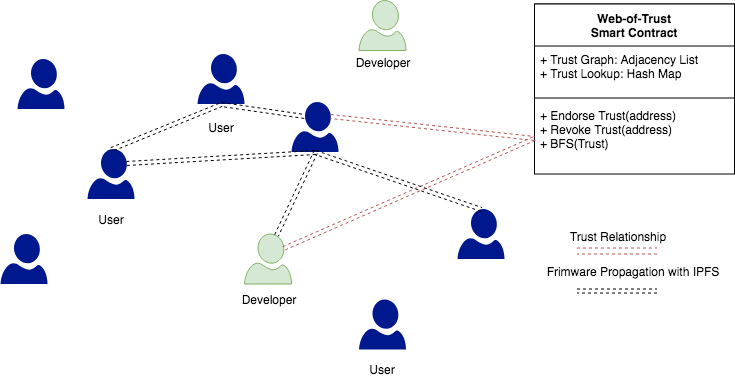
\includegraphics[width=0.95\textwidth]{./pics/IPFS-Archi.png}
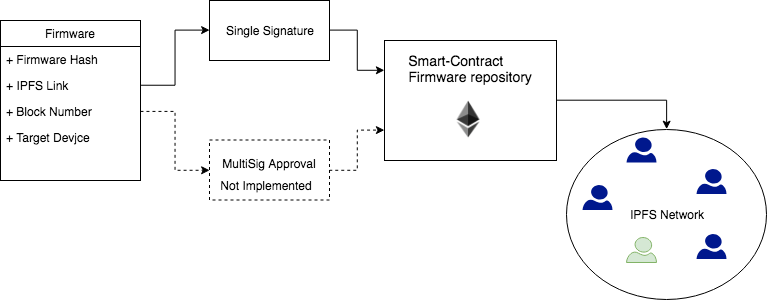
\includegraphics[width=0.95\textwidth]{./pics/Repo-Archi.png}
\caption{Código network architecture diagram. Users are arranged on a graph based on their trust relationship, which is formalized in the Web-of-Trust smart-contract. Firmware metadata are stored on the firmware repository smart-contract and updated using the Código clients. Firmware distribution is on the IPFS layer in which the Código client is uploading/downloading the firmware from the IPFS network.}
\label{fig:arch}
\end{figure}


The first layer of the system lays on top of the Ethereum blockchain. Two smart contracts were developed on top of Ethereum using Solidity \cite{solidity}. At the time of writing Solidity is the only robust language for developing Ethereum Smart Contracts. Solidity is a Javascript type of language that compiles down to Ethereum Virtual Machine instructions that can be executed by the miners. It should be noted that a new language for Ethereum smart contracts, Vyper \cite{vyper}, is also in late alpha stage. The two contracts are independently deployed and communicate with each other using Ethereum transactions. The first contract is responsible for modeling trust while the second is the firmware repository. 

\subsection{Web-of-Trust Smart-Contract}{
The Web-of-Trust smart contract is an implementation of the Web-of-Trust idea in Solidity. The Web-of-Trust is represented as a directed graph and it is implemented using an adjacency list data structure. Nodes can use the web of trust contract independently to allocate their trust to other developers. Figure \ref{fig:webT} illustrates an instance of Web-of-Trust. In this example, Alice trusts Bob with a level 2 trust. Contrary, Bob trusts Alice with a level 1 trust. It is possible and quite likely that the trust graph is not fully connected. For example, in the Web-of-Trust instance in Figure \ref{fig:webT} there is no path from Chloe to Bob. In that case we define Chloe's trust to Alice to be -1. Users are expected to bootstrap their trust profile with the address of other developers that they find from other sources, such as the developers website or GitHub profiles. Then they use the client to allocate their trust towards them. IoT gateways that use the client can bootstrap their trust profile with the address of the manufacturer.

\begin{figure}[!htb]
\centering
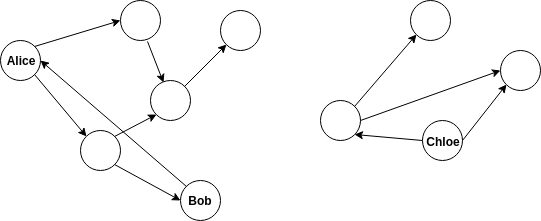
\includegraphics[width=\textwidth]{web_of_trust.png}
\caption{An instance of Web-of-Trust implemented as a directed graph. Trust of party A (vertex) towards B (vertex) is defined as the minimum number of hops (edges) required to reach from A to B. In case no path from A to B exists, we define the trust of A towards B to be -1. }
\label{fig:webT}
\end{figure}

Trust can be allocated to a developer using the endorse trust function of the smart contract. The endorse trust function of the smart contract is performing some logical tests to avoid storing duplicate addresses and appends the new address to the trust graph. As a result, the computational cost of the function and hence the gas cost is independent of the number of trusted users. This is also illustrated in Figure \ref{fig:addTrustGas} that visualizes the gas cost entailed in trusting a new address. It should be noted that in the Ethereum blockchain it more gas is required to change a value from zero to non-zero than from non-zero to non-zero even, if the absolute value difference is the same. As a result, the first call by the user to the function will be more costly. The users have access to the opposite operation which is deallocating trust. The deallocation function needs to iterate over the connections of the users, delete the requested connection and then rearrange the rest of the connections. Therefore the computational cost of the function is $O(trusted\_users)$  and hence the gas cost of the function is increasing linearly in terms of the trusted users. This is also illustrated in Figure \ref{fig:rmTrustGas} that visualizes the gas cost associated with removing the trust from an address. To put the numbers into perspective, with a gas price of 6 GWei, the first call to the endorse trust function would cost 0.00048 Eth, while revoking the trust would cost 0.00033 Eth for a user with 40 trusted addresses.

\begin{figure}[htb!]
\centering
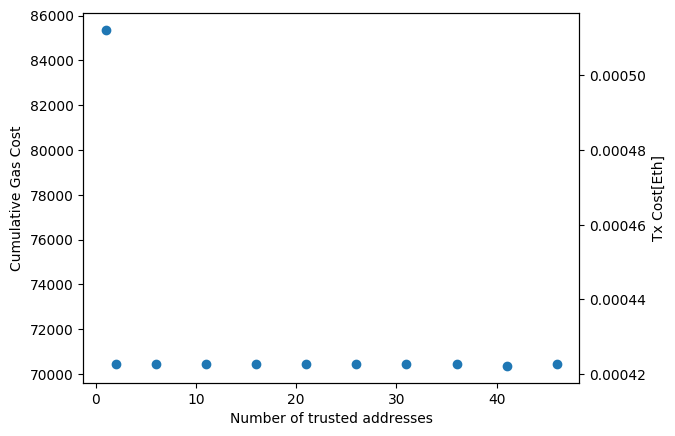
\includegraphics[width=0.95\textwidth]{./pics/endorse_trust.png}
\caption[test]{Gas required and equivalent Eth cost for allocating trust to a user to the Web-of-Trust smart contract.}
\label{fig:addTrustGas}
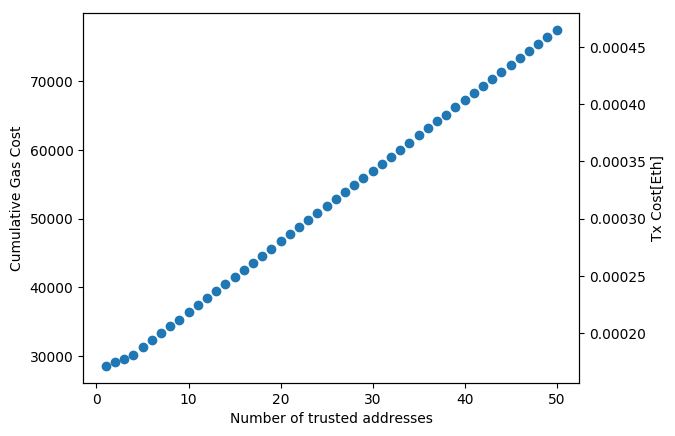
\includegraphics[width=0.95\textwidth]{./pics/revoke_trust.png}
\caption{Gas required and equivalent Eth cost for deallocating trust from a user as a function of the number of trusted addresses to the Web-of-Trust smart contract. Contrary to the trust allocation function, this function transactions costs are linearly correlated with the number of trusted addresses.}
\label{fig:rmTrustGas}
\end{figure}

The last and possibly the most important function of the Web-of-Trust smart contract is the function that calculates the level of trust of user A towards user B. This function does not alter the state of the smart-contract, thus nodes can calculate it locally without the need to perform and consequently pay for a transaction. This function is a classic shortest path graph traversal from origin A to destination B. Theoretically, Djikstra's algorithm \cite{algos} would be the best choice for calculating the shortest path from vertex A to vertex B in a graph with positive edge weights. However, the efficient version of  Djikstra's shortest path algorithm relies on a priority queue data structure. This is a big constrain in Solidity. The reason for that is that custom data structures such as a priority queue are not implemented in the standard library of the language. As a result to use such data-structures one would need to implement them from scratch. The main problem is that in order to use the implemented data-structures one would need to perform a transaction. For example, if someone wants to use their own implementation of a priority queue they would need to create a transaction to initialize a new contract that implements it. This happens even if the custom data structure is used only as a local variable and the function as a whole does not alter the state of the smart-contract. This is due to the fact that smart-contracts, although they syntactically resemble classes they are not. There is no such thing as creating a temporary instance of a contract, operating on it and then at the end of the function deleting the contract instance. As graph traversals are unbounded in size if the function is included in a transaction such operation could result in arbitrarily high transactions cost. Additionally, an attacker could perform the following attack to grief an honest user:

\begin{enumerate}
\item Alice trusts user Eve
\item Alice sends a transaction to calculate her trust towards another user
\item Eve sees the transaction in the mempool and sends multiple transactions to endorse dummy addresses with a high gas price. As a result, Eve's transactions are performed before Alice's.
\item As a result Alice would have to pay more money in transaction fees than she expected in order to perform the requested trust calculation.
\end{enumerate}

Due to the aforementioned reasons, we opted to implement a less efficient traversal method that does not need a priority queue data structure. The traversal is implemented in Solidity using the Breath-First-Search (BFS) algorithm \cite{algos}. The BFS implementation correctness was evaluated with a set of unit tests that checked if the implementation could calculate the trust correctly in the case of cycles in the graph, absence of a path between the destination and the origin and in the case of multiple paths between the destination and the origin.
}

\subsection{Firmware Repository Smart Contract}{
The firmware repository can be thought of as a classic torrent website repository, that is hosted on Ethereum instead of a web-server. The main goal of this smart contract is to store the metadata required to download a firmware. This is a high level requirement that can be translated to a smart-contract, by which developers should be able to upload firmware and users should be able to find all the information they need to download a firmware. In the rest of this section the design of each function of the firmware repository will be discussed. 

Firstly, before going into the details of the smart-contract functions, we must define an appropriate data structure to represent firmware. In Código Network a firmware is represented as struct with the following variables:
\begin{itemize}
  \item  Firmware hash stored as 32-byte array
  \item  IPFS link stored as a string
  \item  Firmware description stored as a string
  \item  Block number stored as 256 bit unsigned integer
  \item  Target device stored as a string
\end{itemize}

The firmware representations follows the guidelines of Code Signing proposed by Cisco \cite{fleischman2002code}. One will observe that there are no signatures of the hash, to validate the author of the firmware. The reason for that is that the signature of the developer is already required by the Ethereum blockchain when he/she uploads the firmware to perform the transaction. Thus it was decided not to store this information in the smart-contract as it already exists in the blockchain. Additionally, the block number is also stored as an indication of the age of the firmware. Assuming that Ethereum maintains the policy of producing blocks at an almost fixed interval, using the block number anyone can calculate at what day the firmware was added to the blockchain.

An improvement that could be made to the current design, which was not implemented during the scope of the project is the introduction of $m-n$ multi-signatures. A group of developers working on the same code-base can publish a smart contract that implements m-n signatures. This behavior is supported by Código Network. Users will merely trust a smart-contract instead of a user address in Web-of-Trust.

In order to upload a firmware to the blockchain, developers need to provide the hash of the firmware, the IPFS link of the firmware, the firmware description and the target device and a PoW nonce. As it was already mentioned, developers need to provide a valid PoW solution in order to upload a new firmware. In general the aim of the PoW system is to allow developers to upload 1-2 firmware updates per day. For each developer, an unsigned integer called challenge, the time of the last submission and the current difficulty are stored. The goal of the developer is to submit a nonce to the smart-contract with the following property:
\begin{align*}
SHA-3(nonce,challenge) \leq difficulty
\end{align*}

The initial PoW difficulty is $10^{77}$ and is divided by $50$ each time a developer pushes a new firmware to the repository within the same day. As the difficulty decreases, the required number of computations increases. If the last proof was submitted more than one day ago, then the difficulty is reseted to its initial value. The challenge is a cryptographic salt that is generated using the following formula:
\begin{align*}
SHA-3(nonce_{prv},challenge_{prv},blockhash)
\end{align*}

Under the assumption that the output of the SHA-3 is uniformly distributed in the range $[0,2^{256}]$, then the probability of generating a valid PoW, $Pr_n[valid|nonce]$, as a function of the number of firmware added, $n$, can be calculated as follows:

\begin{align*}
&initial\_difficulty = 10^{77} \\
&Pr_n[valid|nonce] = \frac{initial\_difficulty}{50^n 2^{256}}
\end{align*}

The $initial\_difficulty$ value was set such that the $Pr_1[valid|nonce] = 0.9$

Furthermore, we can define a set of random variables $Attempts = \{Attempts_n\}$. Each random variable, $Attempts_n$, denotes the number of SHA-3 computations required to calculate a valid PoW if one has added $n$ firmware that day. Each calculation of SHA-3 calculation is a biased Bernoulli trial with probability $p=Pr_k[valid|nonce]$. As a result, $Attempts_n$ is a Geometric distribution \cite{ProbBook}. For each $Attempts_n$ we can calculate the expectated value and variance of the distribution as follows:

\begin{align*}
&\mathbb{E}[Attempts_n] = \frac{1}{Pr_n[valid|nonce]},
&var[Attempts_n] = \frac{1-Pr_n[valid|nonce]}{Pr_n[valid|nonce]^2}
\end{align*}

Based on the formulas above we calculate and present in Table \ref{tab:pow_prob} the expected value and the standard deviation of $Attempts_n$ for $n \in [1,3]$

\begin {table}[htb!]
\caption {The expected number of SHA-3 computations and its standard deviation required to upload multiple firmware within the same day.} \label{tab:pow_prob} 
\begin{center}
 \begin{tabular}{|c| c|c|}
 \hline
 Number of Firmware Added & Average & Std \\ [0.5ex] 
 \hline
  1 & 1.158 & 0.427  \\
  \hline
  2 & 57.896 & 57.394 \\
  \hline
  3 & 2894.802 & 2894.302 \\
  \hline
\end{tabular}
\end{center}
\end {table}

Figure \ref{fig:powCost} graphically illustrates the required SHA-3 computations to upload multiple firmware within the same day under a typical execution. The required SHA-3 computations increase in an exponential rate. Note that the SHA-3 calculations are performed in the client and as a result, the PoW does not increase the transaction costs to add a new firmware by a significant amount.

\begin{figure}[htb!]
\centering
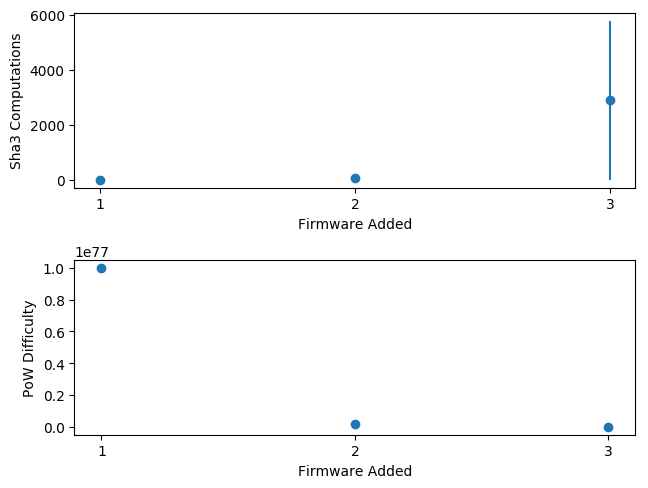
\includegraphics[width=0.95\textwidth]{./pics/pow_cost.png}
\caption{SHA-3 computations required and PoW difficulty as a function of consecutive firmware updates per day. The computation cost increases with an exponential rate as a function of the firmware added}
\label{fig:powCost}
\end{figure}

Each developer is allowed to upload two different versions of the same firmware in the repository, one latest commit version of the firmware and one long-term-support (LTS) version per device type. Although, the number of allowed firmware per developer is two, there is no way to enforce that the latest-lts convention will be followed by the developers. Additionally, developers can use the smart-contract to upload new firmware or edit the description of an existing firmware. Users can query the firmware repository to find a specific firmware, find the firmware from the most trusted developer and find a list of firmware from the most trusted developers. Figure \ref{fig:addGasC} illustrates the transaction costs for adding a new firmware to the repository. The cost is 0.0027 Eth for the first time and the price drops to 0.0009 Eth onwards. In addition to that, there is the extra cost (in terms of CPU cycles and consequently electricity) for finding the appropriate nonce and solve the PoW.

\begin{figure}[htb!]
\centering
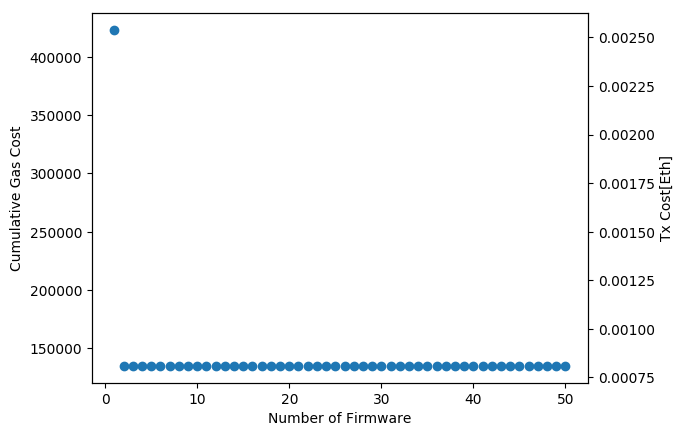
\includegraphics[width=0.91\textwidth]{./pics/add_firmware.png}
\caption{Gas required and equivalent Eth cost for uploading a new firmware to the firmware repository smart-contract}
\label{fig:addGasC}
\end{figure}

}

Users can view and then download the most trusted firmware, or retrieve a list of trusted firmware. These functions merely browse through the smart-contract data without modifying its state. As a result, these functions can be computed without a transaction. This comes with an additional privacy advantage. As users, do not have to make a transaction to download a firmware, then no personal information about the type of devices they own is leaked in the blockchain.

\subsection{Código Network Clients}{
To interact with the blockchain layer and download/upload a firmware from/to the IPFS network, a user and developer client were developed. These clients were designed to make the process of uploading and downloading new firmware smoother in an user friendly way. As a decentralized system, Código network was designed in a away that does not rely on the developed clients to work. The reason for that was to avoid making the clients an implicit centralization point. As a result, the developed smart-contracts are fully autonomous and the user can interact with them with their favorite blockchain enabled tool, without installing the Código client. The same applies to the IPFS layer. Users can use the command-line-interface of the IPFS client directly to download the firmware without relying on the firmware.

To maximize the usability of the client, the option of using remote IPFS and Ethereum nodes is offered. This is particularly useful for IoT devices that do not have the luxury of running a full Ethereum and IPFS node locally. Ideally the user can run an Ethereum and an IPFS node on her computer and then contact those from the IoT devices to perform the calculations. Furthermore, both clients are software applications that rely on the existence of clients that will make the transactions. This means that the clients do not store the private keys of the users nor make transactions themselves. The user would need to connect the client with their Ethereum wallet to perform transactions. This is a responsibility that burdens the user. Finally, both clients were developed using the Python bindings of the Qt framework \cite{summerfield2007rapid}.

The developers client can be used to upload a new firmware directly to the blockchain and to the IPFS. The main benefit of using the developer is that firmware are uploaded to both  Ethereum and IPFS in a congruent way. Figure \ref{fig:devClient} illustrates the developer client UI. The user client is responsible for querying the blockchain to find firmware updates and then download the latest firmware. The user-client also implements the functions of the smart-contracts that do not require transactions. This gives the flexibility to the user to choose between running the smart-contract functions locally on the Ethereum Virtual Machine or making the calculations locally using the client. Figure \ref{fig:userClient} illustrates the user client UI.

\begin{figure}[h!]
\centering
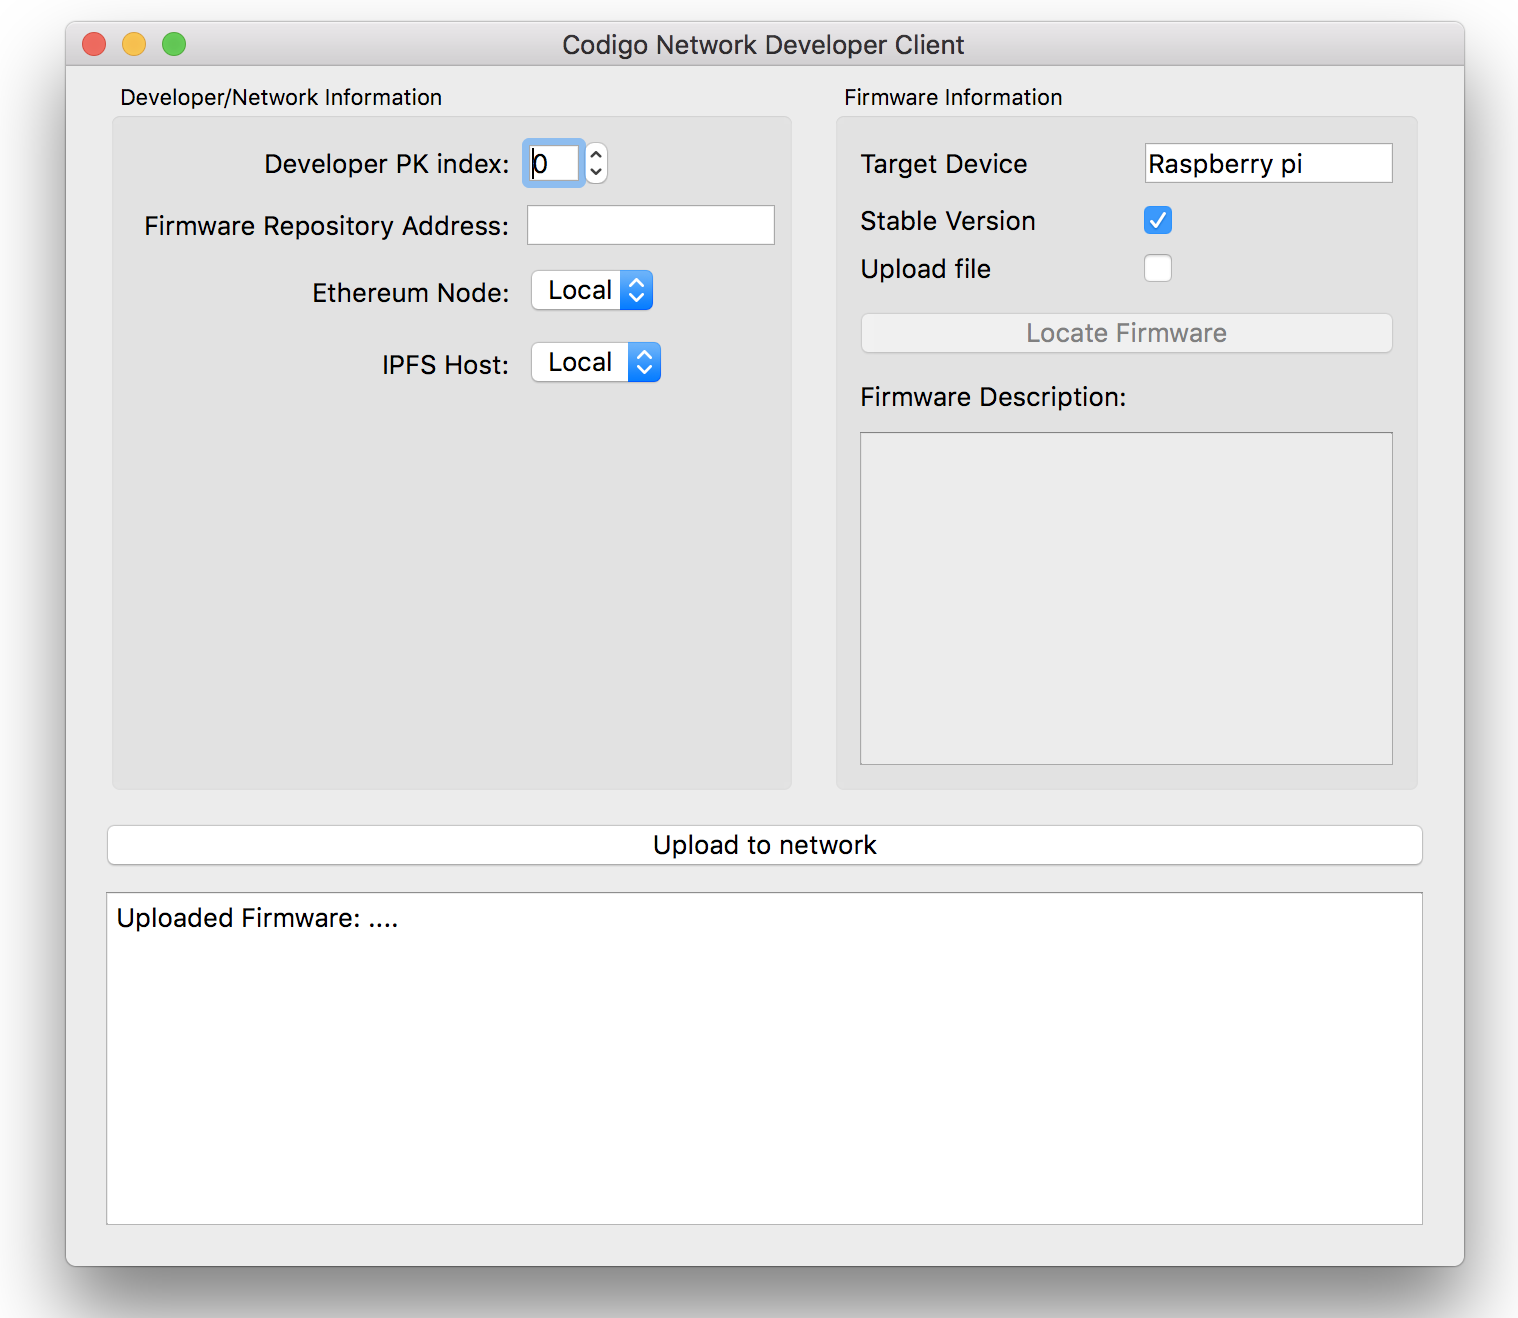
\includegraphics[width=0.95\textwidth]{./pics/Developer_client.png}
\caption{Código Network developer client}
\label{fig:devClient}
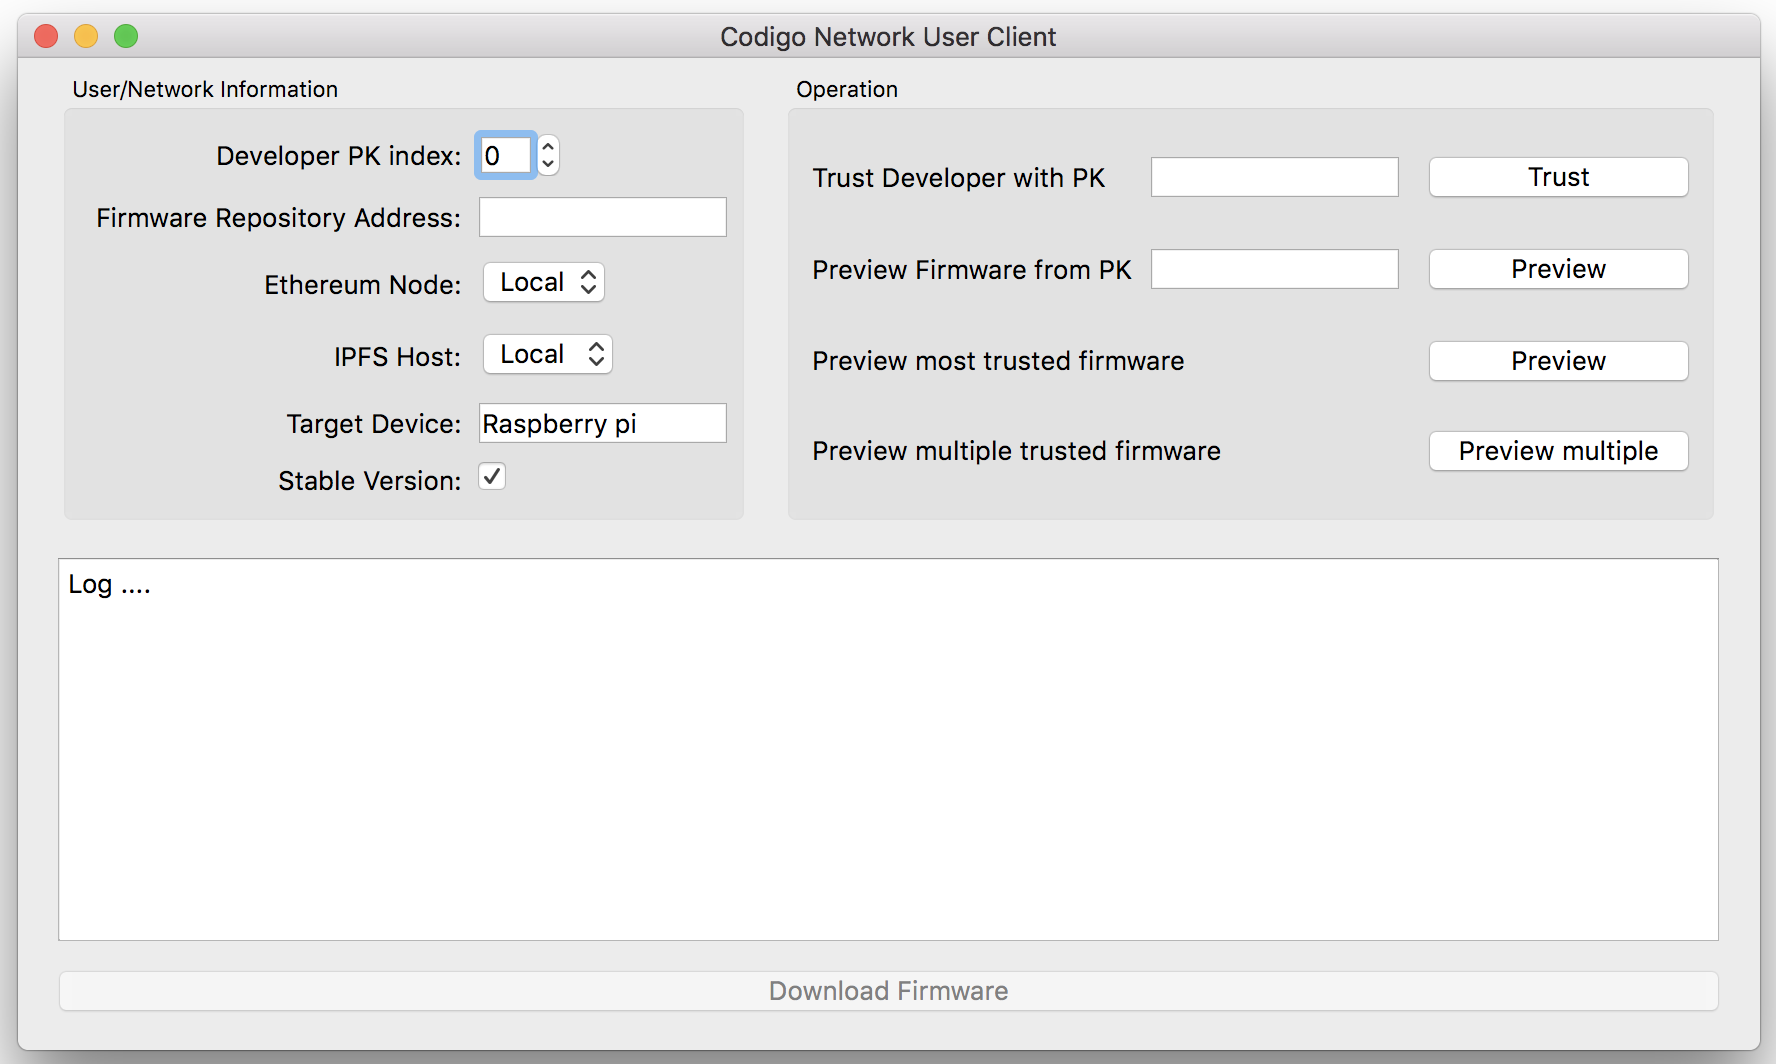
\includegraphics[width=0.95\textwidth]{./pics/user-client.png}
\caption{Código Network user client}
\label{fig:userClient}
\end{figure}
}
}
}